\subsubsection*{Methodology of the ASIC subproject.}

\subsubsection*{Electronics and DAQ: the PETSYS solution}
%
\begin{figure}[!htb]
	\centering
	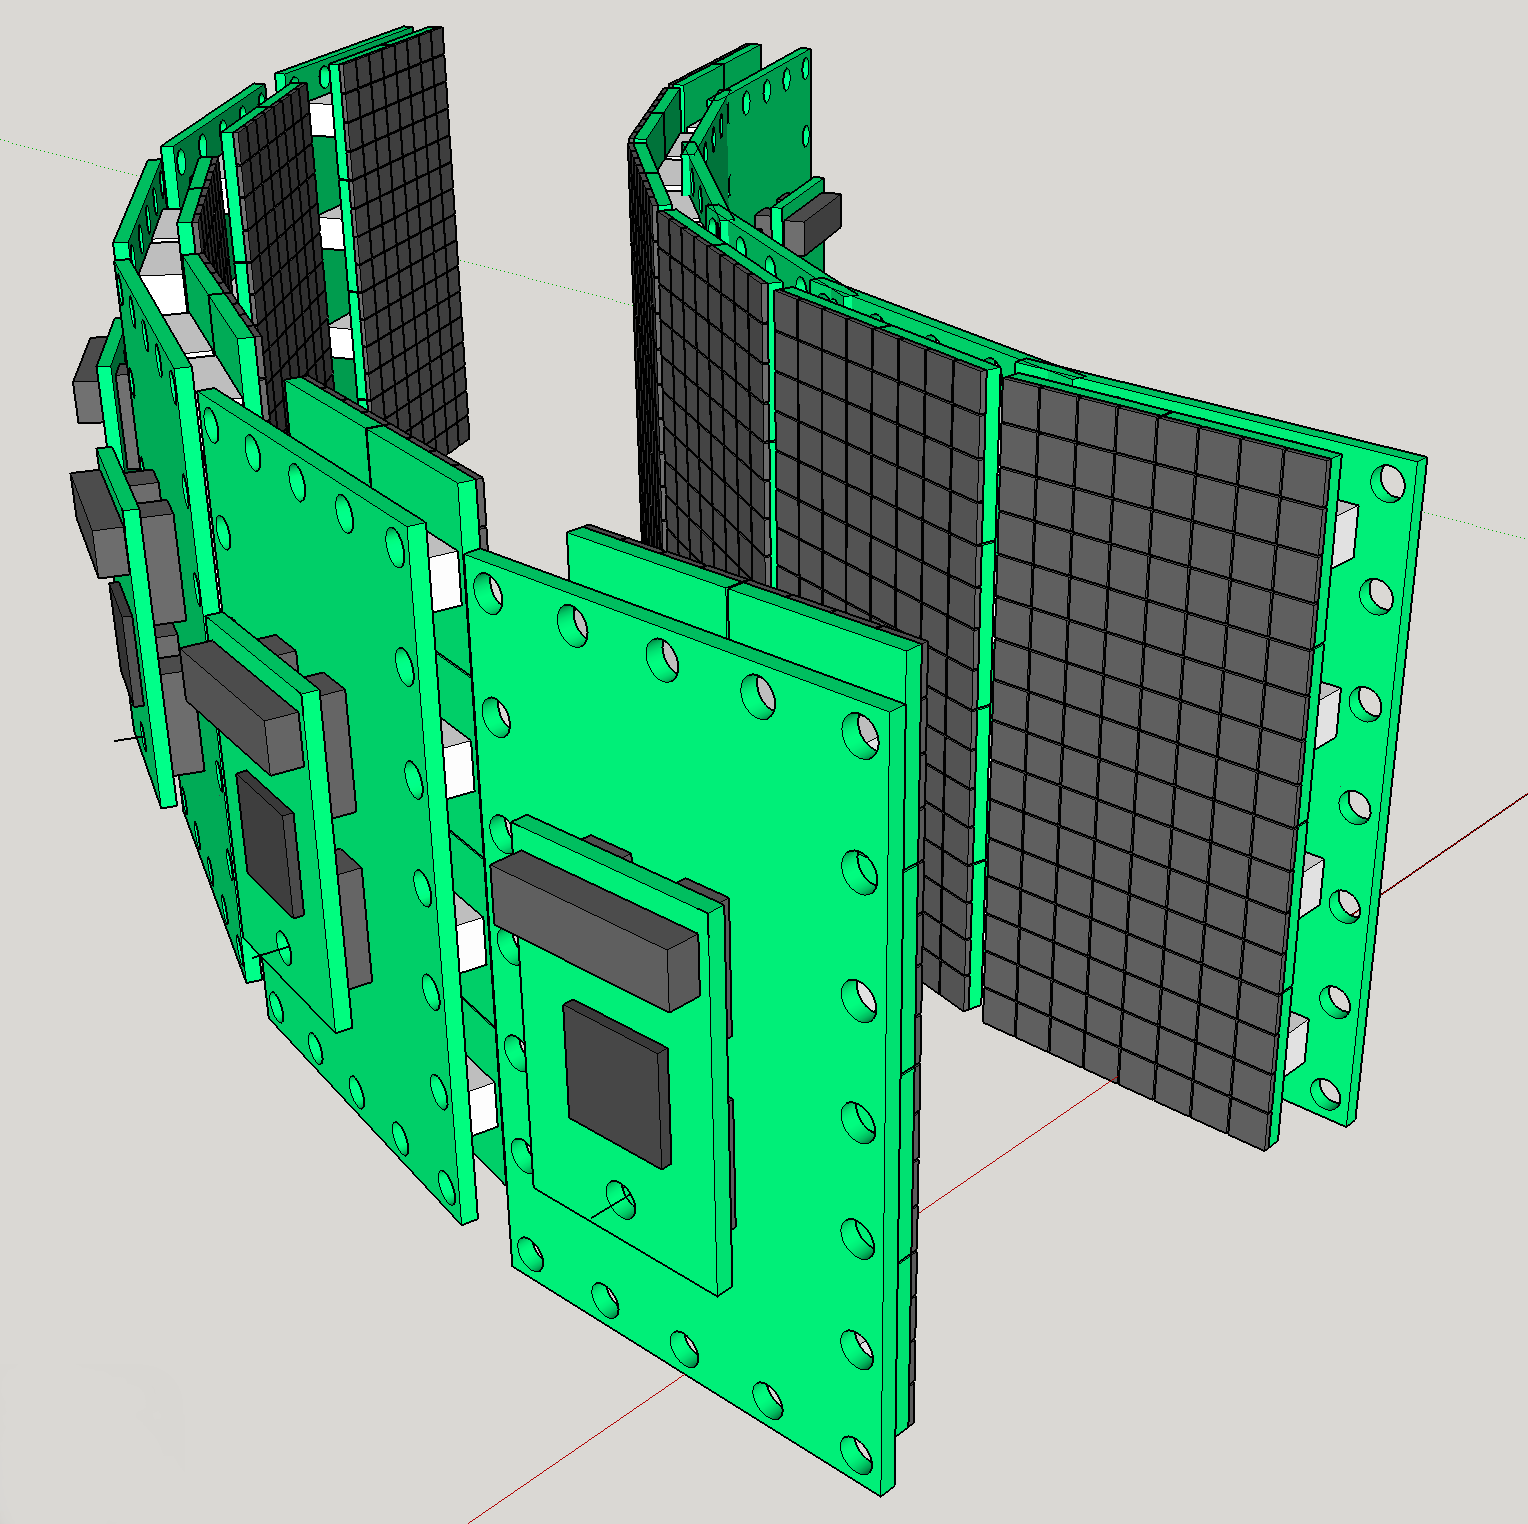
\includegraphics[scale=0.25]{img/PEP.png}
	\caption{\label{fig.pep} A drawing illustrating the arrangement of SiPMs and readout electronics in PEP. }
	\end{figure}

The baseline solution adopted for PETALO is the use of the PETsys TOFPET2 ASIC 
\footnote{http://www.petsyselectronics.com/web/website/docs/products/product1/Flyer\%20ASIC\%20TOFPETv2.pdf}, a low power, low noise SiPM readout ASIC
optimised for  time measurement. The ASIC provides signal amplification and discrimination for 64 independent channels. It uses a low threshold
for  timing and a high threshold for accepting the event. Both thresholds are separately configurable for each channel. When any of the 64 channels exceeds the high threshold the ASIC fires, providing a record giving the channel number, the time and the amplitude of the event. The ASIC has large dynamic range (1500 pC) and can handle large
capacitance (thus large SiPMs), offering a SNR of 25 dB for an
input capacitance of 320pF. A fine TDC binning (25 ps) makes it suitable for CRT measurements in the range
of 100 ps. Each channel can handle a hit rate of 600 kHz, the operation frequency is 200 MHz and the max output
rate is 3.2 Gb/s. The output is fully digital and the power consumption around 10 mW/channel. 

The crucial features of the ASIC are its low time resolution (25 ps) and the low amplifier noise (25 ps for 1 photoelectron signal).   

PETSYS provides a front-end board (FEBA/A) carrying two ASICs, and therefore capable to handle 128 channels. The board dimensions are very compact $52 \times 25.4 \mathrm{~mm^2}$~and fully compatible with the transverse dimensions of the PEP LXSCs ($50 \times 50 \mathrm{~mm^2}$). Thus, each FEB/A can handle a LXSC2 with a double
layer (entry and exit faces) of $8 \times 8$~6 mm SiPMs. If the FEB/A board can be adapted to work at LXe temperatures (it has currently been tested to work at $-80\,^{\circ}{\rm C}$), this allows a very compact readout solution,
as sketched in figure \ref{fig.pep}. Alternatively, one can extract the analog signals of each LXSC using feedthroughs, which have been already developed in the context of the NEXT experiment. 

PEP will deploy 14 LXSCs instrumented with a single matrix of 64 SiPMs (called a Dice Board or DB). Each FEB/A can readout two DBs and therefore 7 FEB/A are needed for the whole system. The low power of the ASIC (about 130 mW per FEB/A) results in a total power dissipation of less than 1 W for the whole system, which is much less of the typical power of a standard cryocooler (about 30 W). 

The FEB/A digital signals are routed to a concentrator board called FEB/D. A single FEB/D can handle up to 8 FEB/A (thus we need only one FEB/D for PEP). In turn, the FEB/D board sends data to a DAQ master board that can handle up to 12 FEB/D master boards (a master FEB/D, in turn, can daisy-chain several slave FEB/D cards). Thus, the adavantage of the solution offered by PETSYS is that is fully scalable to a large system. This would permit a quick upgrade of PEP towards a commercial/pre-commercial system as an spinoff of this project. 

The ASIC subproject will contribute to P2 and PEP fabricating and testing the needed DBs for both prototypes. ASIC is also in charge of procuring, testing and commissioning the PETSYS FEE electronics and DAQ. In addition, ASIC will develop the slow controls of the cryogenic and gas systems. 

\subsubsection*{Developing electronics suitable for LXe temperatures}

VICENTE

\subsubsection*{Studies of fast detectors and electronics for the detection of LXe Cherenkov light}

JJ + Vicente + David
